\documentclass[a4paper,2pt]{report}

\usepackage[a4paper, total={6in, 9in}]{geometry}
\usepackage[table,xcdraw]{xcolor}
\usepackage{pdfpages}
\usepackage{indentfirst}
\usepackage{mathtools}
\usepackage{graphicx}
\usepackage{float}
\usepackage{subfig}
\usepackage{multirow}

\graphicspath{ {./img/} }


\setlength{\parskip}{6pt}

\begin{document}

\begin{titlepage}
    \begin{center}
        \vspace*{3cm}
 
        \LARGE
        \textbf{Instituto Superior Técnico}
        \vskip 0.4cm
 
        \Large{MEEC}
        \vskip 0.2cm

        \Large{Aprendizagem Automática}
        \vskip 3cm
        

 
        \Huge{\textbf{Lab 5}}
        \vskip 0.5cm

        \huge{\textbf{Evaluation and Generalization}}
        \vskip 0.5cm

 
        \vfill
 
        \large
        \textbf{Grupo 9}\\
        \vspace{0.3cm}
        Manuel Diniz, 84125\\
        Alexandre Rodrigues, 90002\\
        
        \vspace{1cm}

        \textbf{Turno:} 4ªf 11h00

    \end{center}
\end{titlepage}

\tableofcontents
\newpage

\chapter{Classificação}

\chapter{Regressão}
    \section{Introdução}
        \par É fornecido um conjunto de dados relativo a imobiliário, com \(13\) \textit{features} não específicadas e um resultado, o preço.
        \par O conjunto de dados fornecido tem uma dimensão relativamente reduzida, com cerca de \(400\) amostras. Para compensar, ao treinar o modelo podemo-nos sentir tentados a treinar por um número de épocas elevado de modo a melhorar o desempenho. Com este método há o risco de do modelo se tornar \textit{overfit}.
        \par De modo a evitar isto, faz-se uso de um conjunto de validação. Após cada época, o modelo é avaliado com este conjunto, e a sua \textit{performance} neste é usada para decidir se o treino deve ser parado ou não. O treino pára se a sua \textit{loss} para este conjunto não decrescer após 50 épocas, e os melhores coeficientes do modelo são restaurados.
        \par Já na regressão é importante escolher uma ordem que aproxime bem os dados, mas suficientemente reduzida de modo a que não ocorra \textit{overfitting}.
    
    \section{Treino da rede neuronal}
        \par De modo a realizar a previsão de preços, estabelece-se, após alguma tentativa e erro, um modelo com quatro camadas, todas elas com ativação \textit{relu}, e com \(32\), \(32\), \(16\) e \(1\) neurónios, por essa ordem. Normalmente a última camada tem ativação línear, mas neste caso é indiferente, visto que não se esperam resultados negativos para o preço.
        \par Como referido anteriormente, o treino é parado antecipadamente após 50 épocas sem melhorias nos resultados. Como métricas são usados o erro absoluto percentual e erro absoluto médios, sendo o segundo também utilizado como \textit{loss}. 
        \begin{figure}[H]
            \centering
            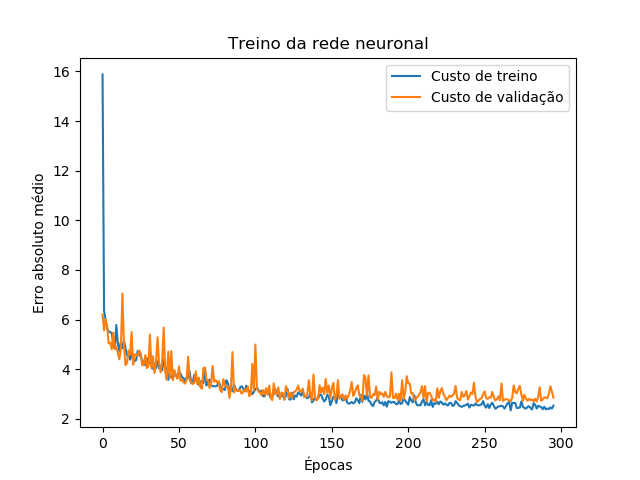
\includegraphics[width = 4in]{training.png}
            \caption{Evolução da \textit{performance} da rede neuronal}
            \label{fig_treino_rede}
        \end{figure}
        \par Como se observar na figura \ref{fig_treino_rede}, o treino pára ao fim de cerca de \(300\) épocas, quando o custo de validação estabiliza.

    \section{Regressão línear}
        \par O outro método de previsão utilizado é a regressão línear, em que o preço previsto é o resultado da soma das multiplicações de cada \textit{feature} pelo coeficiente respetivo, e um \textit{offset}. Sendo que existem 13 \textit{features}, obtém-se 14 coeficientes.
        \par O "treino" neste caso é instantâneo, os coeficientes obtidos através da equação normal. Os resultados estão abaixo.
    
    \section{Comparação de resultados}

        \par Os resultados das regressões estão na tabela seguinte.

        \begin{table}[H]
        \centering
        \begin{tabular}{
        >{\columncolor[HTML]{C0C0C0}}c |c|c|}
        \cline{2-3}
        \cellcolor[HTML]{FFFFFF} & \cellcolor[HTML]{C0C0C0}\begin{tabular}[c]{@{}c@{}}Erro absoluto\\ percentual médio\end{tabular} & \cellcolor[HTML]{C0C0C0}\begin{tabular}[c]{@{}c@{}}Erro absoluto\\ médio\end{tabular} \\ \hline
        \multicolumn{1}{|c|}{\cellcolor[HTML]{C0C0C0}Rede neuronal} & 13.7894\% & 2.6816 \\ \hline
        \multicolumn{1}{|c|}{\cellcolor[HTML]{C0C0C0}Regressão línear} & 17.3136\% & 3.3005 \\ \hline
        \end{tabular}
        \label{tab_regr}
        \end{table}

        \par Devido ao conjunto de dados reduzido, e ao problema em geral, que não ilustra uma ciência exata, obtém-se um erro não insignificante na regressão. No entanto, é bem aproximado o suficiente para generalizar e obter aproximações. Não existe uma diferença muito significativa entre a \textit{performance} dos dois métodos, sendo que a regressão línear já é bem aproximada. Isto sugere uma regressão polínomial provavelmente estaria a par da rede neuronal, com um custo computacional inferior, sendo que seria talvez uma boa escolha.
        \par Mais uma vez, na hipótese de se usar uma regressão polinomial há que ter o cuidado de selecionar uma ordem não excessivamente elevada. Tendo em conta o tipo de dados, uma ordem entre \(3\) e \(5\) seria certamente suficiente.
\end{document}
 